\documentclass[11pt,a4paper]{article}
\usepackage[utf8]{inputenc}
\usepackage{amsmath}
\usepackage{amsfonts}
\usepackage{amssymb}
\usepackage{graphicx}
\usepackage{todonotes}
\usepackage{url}
\graphicspath{{images/}}

\author{Garibaldi Pineda Garc{\'i}a}
\title{Report 15-11-2018}
\begin{document}
  \maketitle
  I arrived to the group on the 15th of November 2018; I've been settling in. 
  I almost have a fully working desktop computer (21-11-2018)!
  
  The objective is to make use of the BrainScaleS neuromorphic platform to do object recognition. 
  For this we will pursue odour identification taking inspiration from insect neural anatomy. 
  
  \section{Background reading}
    \subsection{Layman's introduction}
    I read the Wikipedia entry on insect olfaction as a layman's introduction to the subject. 
    It mainly explains the structure of the olfactory pathway of an insect's nervous system. 
    \begin{figure}[htb]
      \begin{center}
        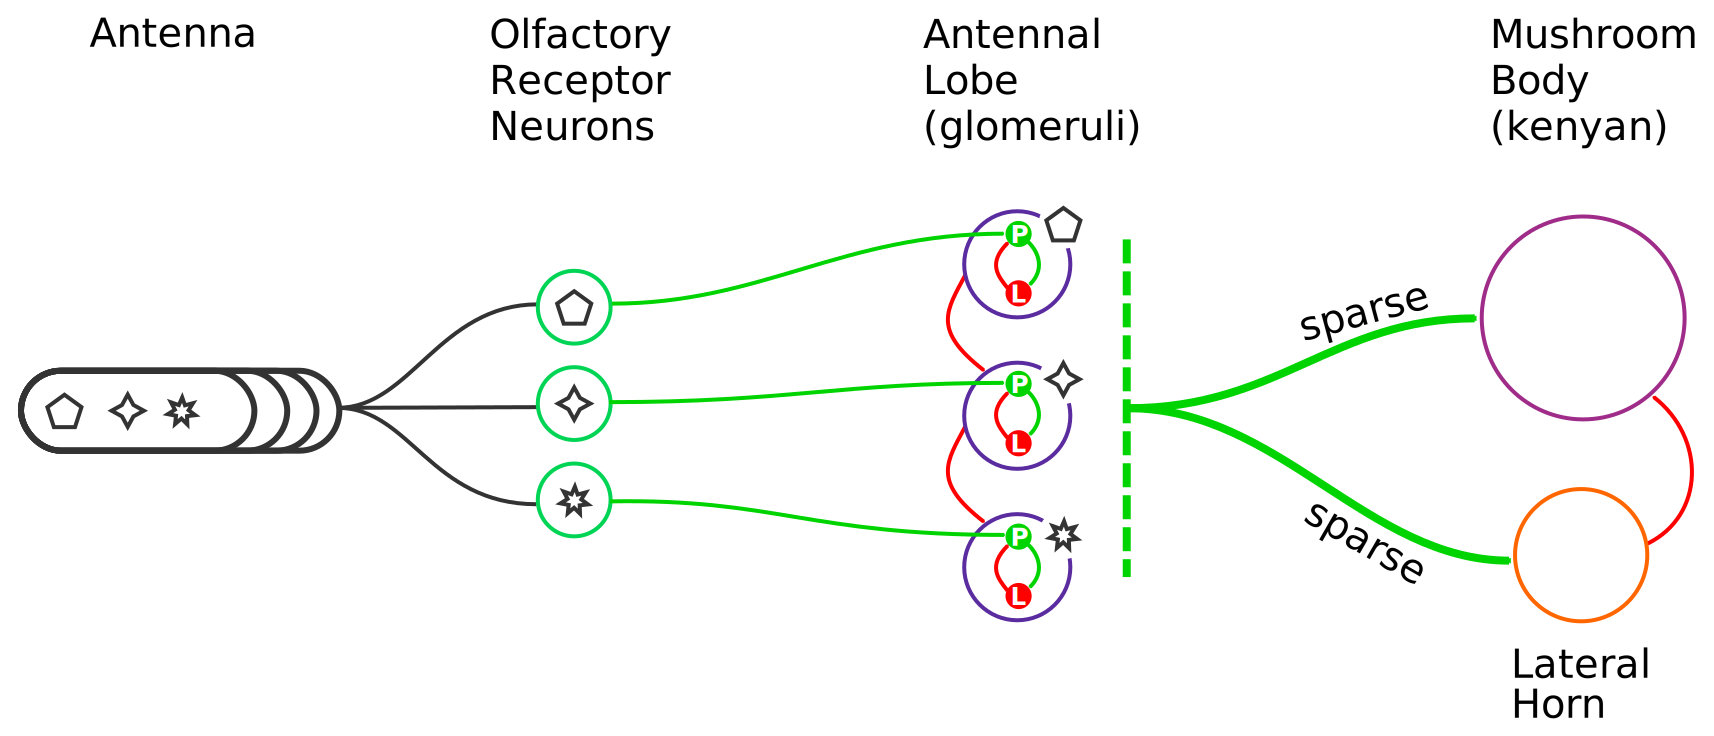
\includegraphics[width=0.7\textwidth]{olfactory-pathway}
      \end{center}
    \end{figure}
    
    \todo[inline]{Is some topological order kept through different layers? This could allow us to introduce distance-dependent connectivity rules.}
    

  I've started reading papers suggested by Mario Pannunzi:
  
    \subsection{Odor plumes and how insects use them}
    The authors describe the complexity of odour plumes and present a review of models. 
    There are 3 different aspects to the full plume structure model:
    \begin{itemize}
      \item Large scale. 
      This deals with the shape and odour strength (average). 
      Many models have been suggested for the direction aspect of the shape ranging from linear to wave-like. 
      Average strength is usually modelled as having an exponential decay with respect to distance.
      Insects use this aspect to orient themselves while finding the source. 
      
      \item Small scale. Odour concentration fluctuation; affects insect instantaneous response.
      Since the medium is turbulent, concentration changes along the plume. 
      Furthermore, insects' behaviour is modified depending on how dense the odour is (e.g. attraction vs. repulsion). 
      
      \item Time-average. How likely is an insect to smell the source.
      
    \end{itemize}
    In summary, odour perception is a complex problem as the signal is propagated through a medium (wind) which is usually turbulent. 
    The signal is thus unreliable and the medium does not commonly indicate the source's direction.
    Nonetheless, insects are able to locate stimuli emitters and react.
    \todo[inline]{Are we skipping this part in the simulation? We just assume antennas received a concentration X of odour Y?}

    \subsection{Learning pattern recognition and decision making in the insect brain}
    Synapses in the mushroom body experience changes which are thought to be linked to odour conditioning.
    Competition between output neurons encourages sparsity; there is evidence of strong lateral inhibition.
    Plasticity from AL to MB to encourage sparsity could lead to reduction of information for KC.
    There must be a balance of sparse activity to cope with information preservation stability and discriminator ability.
    The MB integrates information from other senses not just from olfaction.
    The learning behaviour of output neurons in MB could be equivalent to SVM.
    AL could be doing signal conditioning, feature extraction, decorrelating.

    \subsection{Molecular Architecture of Smell and Taste in Drosophila}
    Lots of chemistry/molecule interaction stuff -- a bit out of my league for now!
    Neuron counts and connectivity ratios are presented (for drosophila fly):
    \begin{table}[h]
      \renewcommand{\arraystretch}{1.3}
      \begin{tabular}{c c c c}
        source & target & ratio & count\\
        \hline
        ORN    & AL     & 30:1 & 1300 ORN\\
        AL     & PN     & 1:3 & 150 PN (43 AL)\\
        PN     & MB     & 1:15 & 2500 MB (100s glomeruli)
      \end{tabular}
    \end{table}

%%%%%%%%%%%%%%%%%%%%%%%%%%%%%%%%%%%%%%%%%%%%%%%%%%%%%%%%%%%%%%%%%%%%%%%%%%

  \section{Using BrainScaleS}
 
  Most required documentation can be found at HBP Neuromorphic platforms guidebook
    \footnote{
    \url{
      https://electronicvisions.github.io/hbp-sp9-guidebook/pm/using_pm_newflow.html
    }
  }
 
  \subsection{Registration to HBP portal}
  To use the system remotely as a ``standard'' remote user we must first register to the HBP Collaboratory via invitation (from a member or sending an intention letter).
 
  After this, one must sign and email back the HBP Platform User  Agreement
  \footnote{
    \url{
      https://www.hbpneuromorphic.eu/UserAgreement_HBPNeuromorphicComputingPlatform.pdf
    }
  }
  Once access has been granted the platform provides test Jupyter Notebooks for the different neuromorphic systems. 
  Collab requires user to authorize the ``Neuromorphic Computing Platform'' to access info in browser so that sub-systems work correctly.
 
  \subsection{Creating and submitting jobs}
  Jobs are coded using PyNN and can be submitted through the browser or a Python web API.
  Creating a Collab is done through a Jupyter-like form (it does not automatically redirect to the newly-created Collab!)
  Installing the web API can be done through pip (requires web access) or setuptools (after downloading the project file).
  Access to different levels of usage of servers can be obtained by submitting a form explaining the intended use of the resources.
  Since the PyNN API version 0.7 (can be obtained through Github
    \footnote{\url{https://github.com/NeuralEnsemble/PyNN/releases/tag/0.7.5}} 
  or PyPi 
     \footnote{\url{https://pypi.org/project/PyNN/0.7.5/}}
  ) is used to interact with the BrainScaleS platform, Python 2.7 is required.
 
  \underline{The work-flow gets tiring after a few tests.} 
  My intuition is that the portal is intended for submitting jobs once the script has been tested on a local machine. 
 
  \subsection{Testing on a local machine}
  To test our programs we have two options: use an old version of NEST or Heidelberg's Docker.io image with a hardware simulator.
  The NEST simulator stopped supporting PyNN 0.7 several versions ago, thus a special configuration is required;.
  It seems the Docker.io image has all tools installed in itself so it's a fast way of starting testing; unfortunately, the \underline{runs are much slower} thus parametrization of each script will be a must!
 
 
 
 
\end{document}

